\newpage
\tikz[remember picture,overlay] \node[opacity=1,inner sep=0pt] at (current page.center){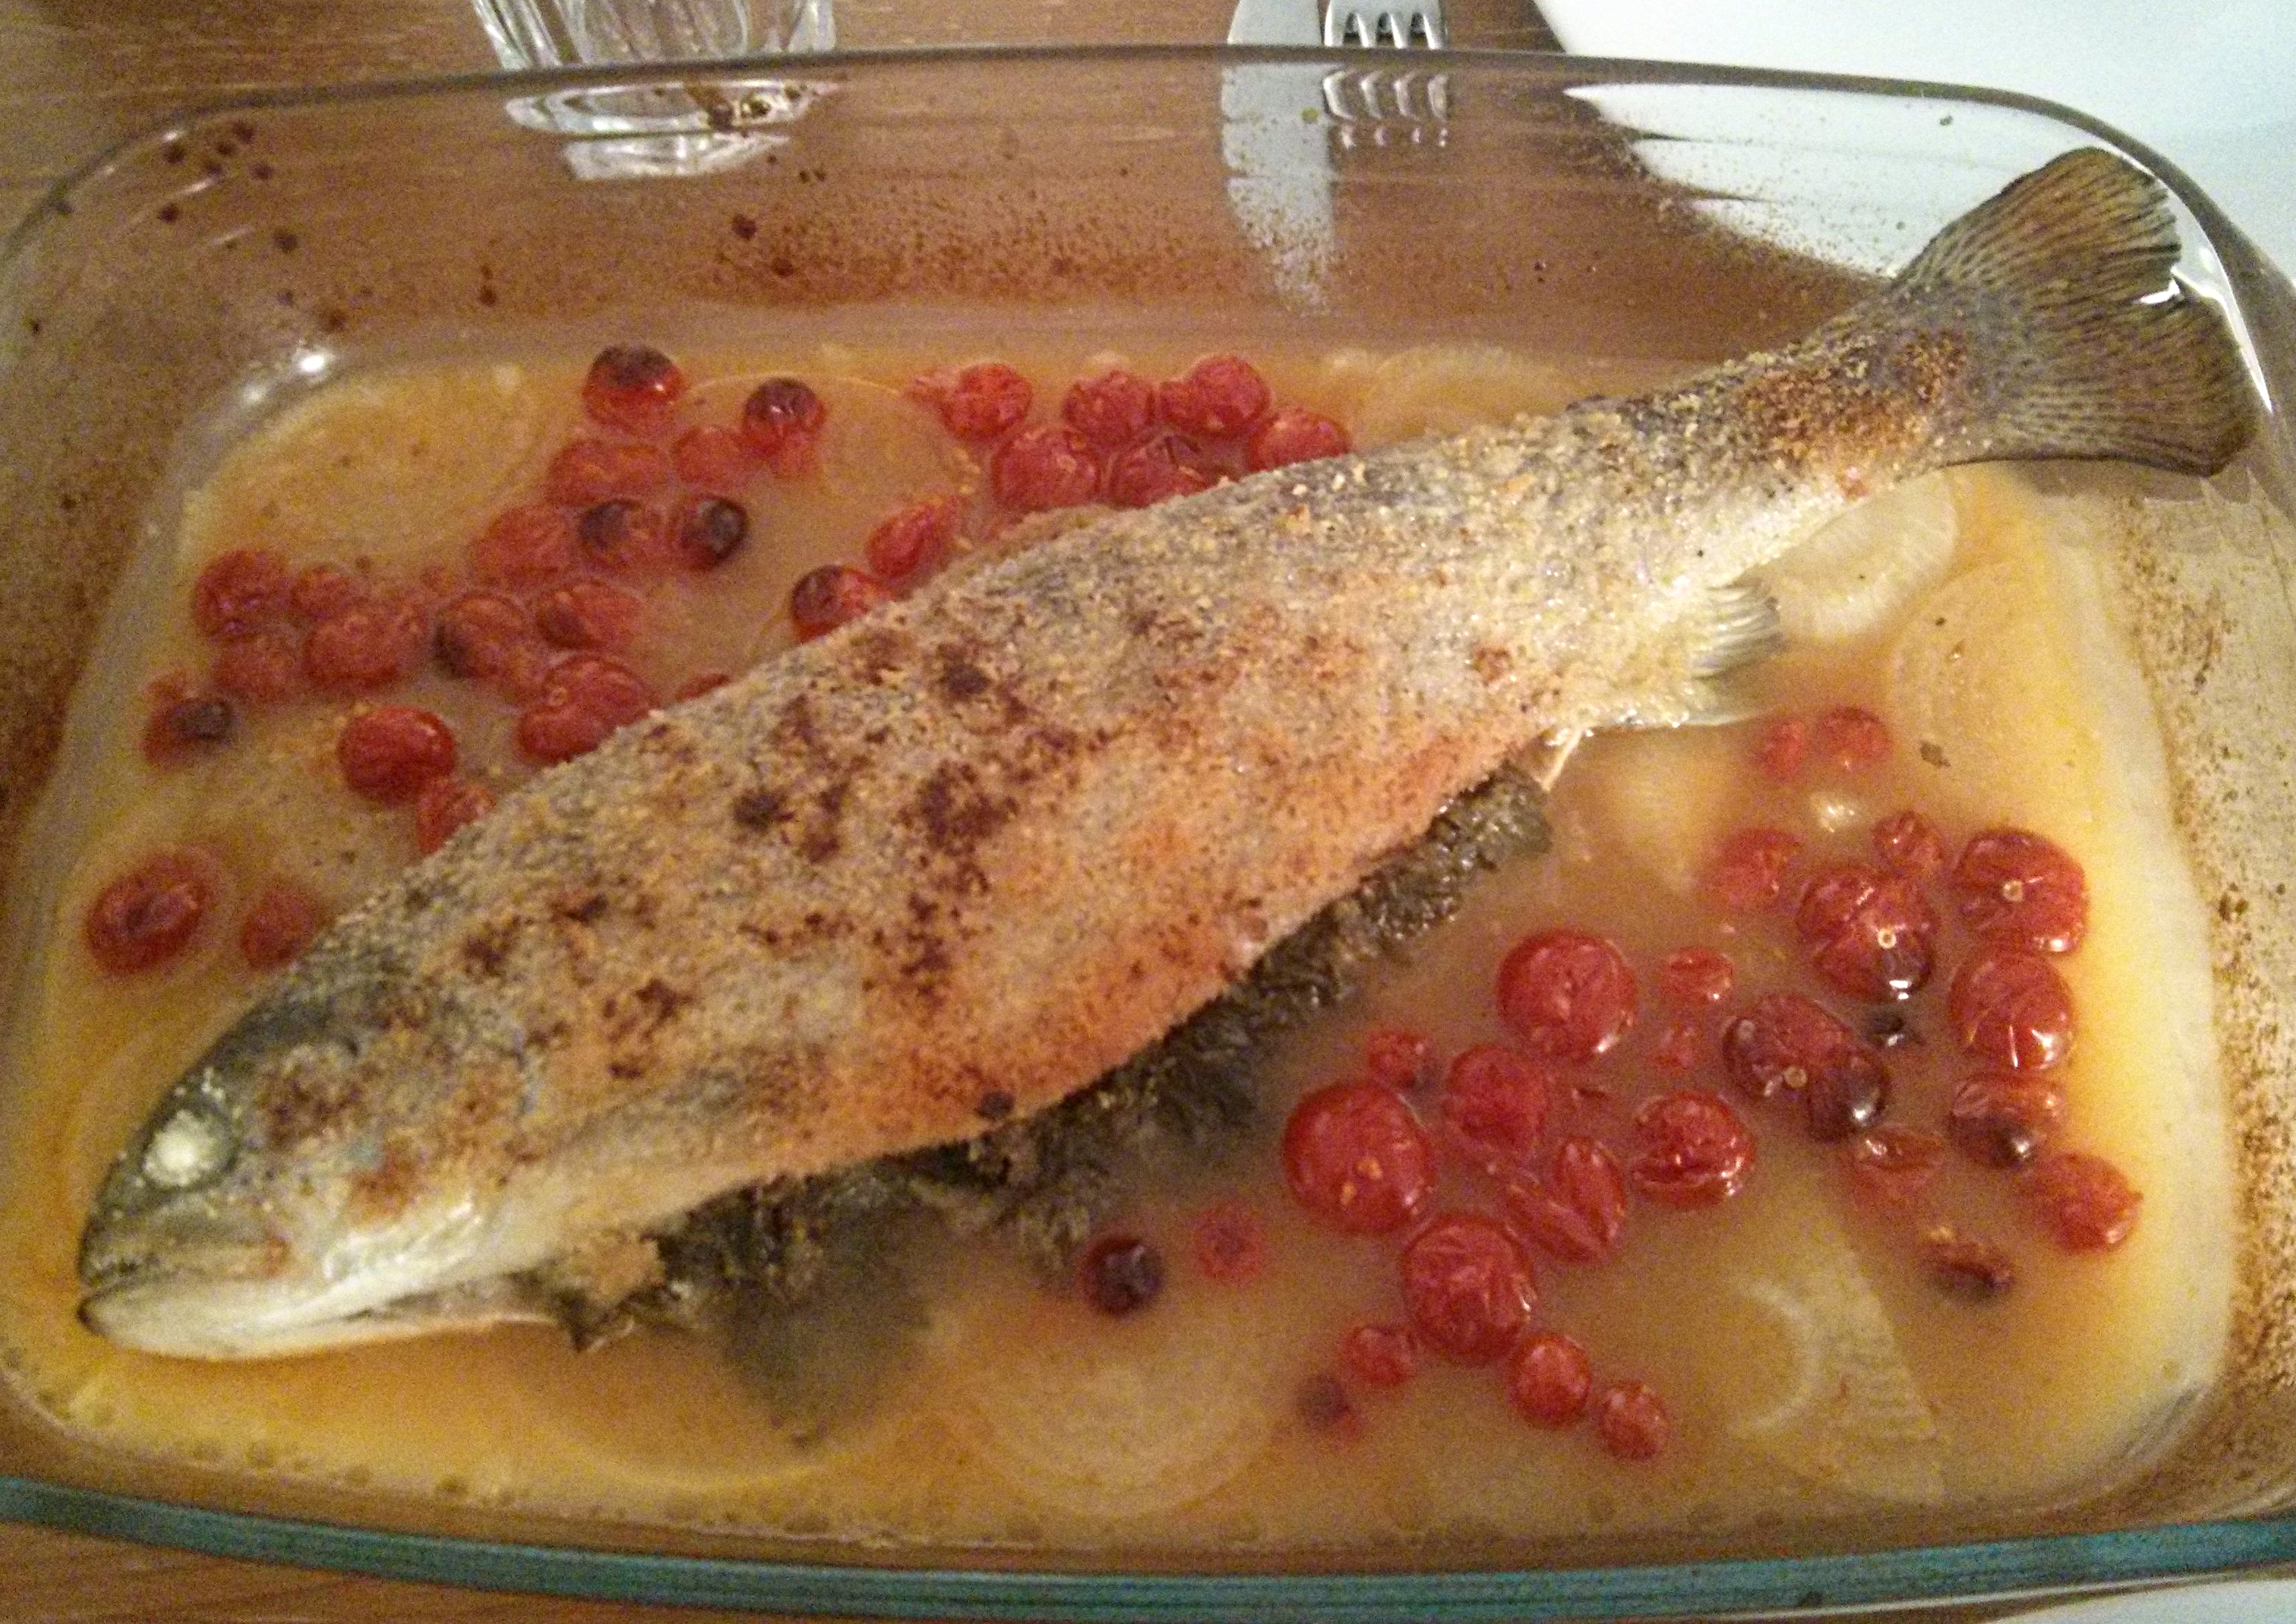
\includegraphics[width=\paperwidth,height=\paperheight]{./bilder/gebackene_forelle_ratio.jpg}};

\begin{recipe}[]{Gebackene Forelle} %Quelle
	\timerecipe[Minuten]{ca. 15+40 } %mit [EINHEIT]
	\personcount[Forelle]{1} % mit[ART]
	\ingredient{1 frische Forelle} % ggf. \nicefrac{1}{2}
	\ingredient{2 Zwiebeln}
	\ingredient{1 Bund Petersilie}
	\ingredient{0,25l Weißwein}
	\ingredient{0,25l Brühe}
	\ingredient{Zitronensaft}
	\ingredient{Semelbrösel}
	\ingredient{75g geschmolzene Butter}
	\ingredient{Salz}
	\ingredient{Pfeffer}

\step
\textbf{2 Zwiebeln} in Ringe schneiden und \textbf{1 Bund Petersilie} waschen und zupfen. \textbf{Forelle} waschen und mit Zwiebeln und Petersilie füllen. 

\step
Forelle in Auflaufform legen und mit \textbf{0,25l Weißwein}, \textbf{0,25l Brühe} und \textbf{Zitronensaft} übergießen. \textbf{Salzen} und \textbf{pfeffern} und mit \textbf{Semelbröseln} bedecken. \textbf{75g geschmolzene Butter} darüber träufeln.

\step
35-40 Minuten bei 200-220°C auf der 2. untersten Schiene backen.

\tippbox{\textbf{Tipp:} Es kann auch weiteres Gemüse, wie beispielweise Tomaten mitgegart werden.} % Tipp in extra Rahmen
\end{recipe}